\chapter{OSNMA: Receiver Operations}
\label{ch:osnma_operations}

In this chapter we'll describe a possible state machine for a receiver that
supports OSNMA. We make the assumption that the receiver CPU is single core and
single threaded. That is, we'll describe a purely sequential and synchronous
state machine that doesn't involve any form of concurrency. The input of this
state machine is the decoded navigation message. In other words, we are not
concerned here about the operations of the receiver's radio frontend, but just
of those of the data processor, and specifically we're interested in
understanding how the authentication operations affect the complexity of a
receiver's firmware.

A first discrimination a receiver should do is if in its current state the
amount of information it holds is sufficient to guarantee it only receives
legitimate data. This amounts to having an authenticated key of the current
chain and knowing that the last period of inactivity doesn't go beyond the
threshold calculated as in the previous chapter. In the first case the receiver
can proceed to receive and authenticate the navigation message, and to solve the
PVT equations with the authenticated data. If not, the receiver must enter a
bootstrap phase where the conditions described above are met.

\section{Authentication bootstrap}
As part of this phase, the receiver needs to bring itself to meet two
conditions, or fail if that's not possible: a root key is present, and the clock
is guaranteed to not have drifted too much since the last synchronization. These
two conditions are independent, but we'll see later that in order to synchronize
the clocks an authenticated key must be in possession of the receiver already.

A procedure to bring the receiver in a state where authenticated navigation is
possible is as follows:
\begin{itemize}
  \item first the receiver should check the presence of an authenticated key in
    its permanent storage. Should the key be absent, the receiver can proceed
    with the next step; otherwise, it can proceed with verifying the clock drift
  \item verify that the chain in force is not in the EOC (End Of Chain) state,
    in which case the receiver should wait to receive the root key for the next
    chain in force as it cannot distinguish if Galileo is sending the root key
    for the ending chain or the root key for the new chain
  \item verify that the chain is not being revoked, in which case the receiver
    should wait until the new root key is sent, identified by a combination of
    \textit{NMA status} and \textit{Chain status} of "Operational" and "CREV".
  \item read the HKROOT: here the receiver builds up all the information contained
    in the HKROOT section. This is important for two reasons: get the root key
    that will allow to bootstrap the auhtentication process, and read the system
    parameters that will be used throughout the whole session
  \item authenticate the KROOT: this is done by using the public key identified
    by the public key ID in the headers section to hash a message containing the
    KROOT, as described in \cite{osnma}, section 5.1
    \begin{itemize}
      \item if the verification succeeds, then the authenticated key is marked
        as such and stored in permanent memory together with the other
        information contained in the header, and the receiver can proceed to
        the next step
      \item if the verification fails, then depending on how stringent the
        security requirements are, the receiver could either proceed to 
        solving the navigation problem without authentication, or abort its
        operation. In either case a notification should be sent to the end user
    \end{itemize}
  \item at this point clock drift should be checked. Based on nominal clock
    precision, key size as defined in the \textrm{KS} field of the NMA header,
    and Equation~\ref{eq:drift_threshold} the receiver should estimate for how
    long it could stay safely offline.
    \begin{itemize}
      \item if the difference between current time and the last time it
        connected to Galileo (which should have been stored) is below the
        threshold for normal operations (i.e. keys sent just after the
        corresponding MAC), the receiver is safe to step into receiving and
        authenticating navigation data.
      \item if not, a procedure of clock synchronization using SLMACs should be
        initiated, which we'll describe next. Once this procedure is completed
        and clock drift has been restored to a level where standard
        authentication operations are safe, then the receiver should step into
        the navigation state.
    \end{itemize}
\end{itemize}

\begin{figure}[h!]
  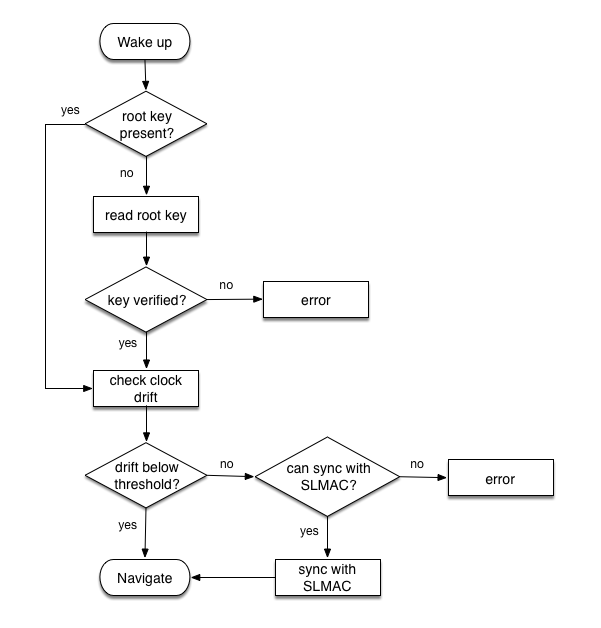
\includegraphics[width=\linewidth]{figures/flowchart_bootstrap.png}
  \caption{Decision tree for OSNMA authentication bootstrap}
  \label{fig:flowchart_boostrap}
\end{figure}

\section{SLMAC clock synchronization}
If the offline period has been too long to guarantee that the security condition
is met for keys that are sent just after the corresponding MAC, the receiver can
try to reduce the drift by reading the GST information from a subframe that is
being authenticated using a SLMAC. This can be done after the receiver has
verified if the security condition for SLMAC holds:
\begin{itemize}
  \item the receiver should first verify if its offline period allows to trust
    keys delayed by \num{30}\si{s}
  \item if this is not the case, then the receiver should check if the offline
    period allows to trust keys delayed by \num{300}\si{s}
  \item if none of these conditions are met then OSNMA cannot be safely used.
    Depending on how the receiver is configured it should either abort its
    operations or continue by solving the navigation problem without
    authenticating the data. In either case a notification should be shown to
    the end user
\end{itemize}

Once the receiver has determined which key delay meets the security constraint,
it should initiate the clock synchronization procedure as follows:
\begin{itemize}
  \item first, it should keep reading subframes until a MAC with an ADKD value
    of 11 or 12 is transmitted (depending on the key delayed identified:
    \textrm{ADKD=11} for \num{30}\si{s} delay, \textrm{ADKD=12} for
    \num{300}\si{s})
  \item while reading subframes, the receiver should keep track of the GST
    values read in WT5 (GST WN and GST TOW as described in \cite{galileoicd}).
    Together with this, the receiver should mark the time at which the GST was
    received (i.e. the local time of beginning of the subframe reception).
    This is important as the receiver must be able to account for the time that
    pass between advertisement of GST and the actual clock synchronization
  \item once the MAC with ADKD set to 11 or 12 has been read, the receiver must
    wait either 1 or 10 subframes, and then read the key being transmitted at
    that time
  \item once the key has been received, it can be authenticated against the
    latest authenticated key stored in permanent memory (it being the root key
    or any other more recent key that has been verified against the root key).
    This is done by applying the selected hash function a number of times as
    described in the authentication bootstrap paragraph above
  \item if the key is successfully verified, the receiver can proceed to
    synchronize its clock with the GST it read \textit{while reading the
    authenticated key}. Authentication of the GST is guaranteed by the fact that
    the advertised GST is directly used to compute the key index, so a forged
    timestamp would result in the key not being verified. At the same time, the
    receiver should overwrite the last authenticated key in permanent storage
    with the one just verified, to help speeding up authentication of subsequent
    keys. Once the clock is synchronized, the receiver can step into the
    navigation state
  \item if the key cannot be verified, depending on its settings, the receiver
    should either abort its operations or proceed to the navigation state with
    disabled authentication. In either case the end user should be notified.
\end{itemize}

\section{Authenticated navigation phase}
If the receiver has made sure of complying with the security condition of TESLA
it can enter the navigation phase. The goal of this phase is to solve the PVT
equation using authenticated data received from satellites. For this to be
accomplished the navigation message needs to be received from a number of
in-view satellites, together with their authentication codes and the keys that
generated them. Given the nature of how data is transmitted, two aspects need to
be considered. First, an efficient way to store and access the data just
mentioned that accounts for piece-wise reception of information. Second, a state
machine to process the received data and handle error cases.

\vspace{\baselineskip}

To understand the problem of storing the data related to the navigation message
and its authentication, it's useful to analyze the lifecycle of these two
components. Starting from how OSNMA groups data to be authenticated with a
single MAC, we distinguish three main categories: ephemeris data, almanac data
and Galileo-GPS conversion parameters. In a 30s cycle, the navigation message
includes all the ephemeris for the transmitting satellite, the conversion
parameters, and almanac data for one and a half satellites out of 36. In the
same time frame, depending on the configuration, 1 to 15 MACs can be
transmitted.  This means that in some cases the receiver could receive data in a
subframe and its authentication in a subsequent subframe, or the other way
around. In any case this means that the receiver needs to have a local cache
that captures the following:
\begin{itemize}
  \item authentication parameters contained in the HKROOT header section
  \item individual navigation message fields
  \item authentication codes, their associated time and position within a
    subframe
  \item keys associated to the authentication codes
  \item status of the validity of a key
  \item status of the verification of an authentication code
\end{itemize}
The navigation message fields amount at least to:
\begin{itemize}
  \item ephemeris for 36 satellites
  \item almanac for 36 satellites
  \item remaining bits of a subframe that are not captured by other fields
\end{itemize}
In case the receiver is capable of receiving GPS signals and wishes to
authenticate them, then the storage requirement includes also the authentication
codes relative to the GPS navigation message, for all the possible 35 GPS
satellites Galileo can authenticate.

One important aspect to consider that might affect the efficiency of the storage
mechanism is the fact that one authentication code applies in general to more
than one field. To avoid duplicating the authentication codes for each field, a
pointers-based structure might be implemented, in which for each field just a
pointer to the data structure storing the actual MAC and contextual timing and
position information is stored.

Another important tradeoff that must be considered when designing the storage of
the receiver is related to the fact that Galileo can authenticate also a whole
full subframe; here the two opposing forces are memory and complexity. On one
side, one could allow for a complete copy of the subframe to be stored
independently from the other fields. The second approach is to collect the bits
of the subframe that are not included in the other stored fields, and have the
CPU recompute the subframe structure prior to authentication. This last approach
has the advantage of saving memory, but requires some computation on the
processor side before the subframe could be authenticated. The first approach
instead removes the need of CPU cycles at the expense of more memory used and
some duplicated data. On the other hand, this approach also allows the receiver
to store ephemeris and almanac data independently from the data received in the
last subframe (e.g. the receiver might keep a verified version of the individual
fields for use in the PVT solution, and at the same time authenticate the last
subframe with the option of discarding it in case authentication fails without
losing already verified data).

\vspace{\baselineskip}

Once the data structure is defined, it's useful to discuss how the receiver
should fill the actual data in. In general it's important to realize that some
of the data presented above needs to be computed by the receiver, which needs to
make sure enough CPU cylces are scheduled at the right time, without running
into the risk of blocking other operations. From this point of view, one
approach is to perform data processing operations only at the boundaries of
logical parts of the navigation message, namingly at the end of a page, at the
end of a subframe or at the end of a frame, as suggested in
\cite{galileo_book}. Processing the navigation data at the end of a
\num{2}\si{s} page has the potential advantage of making data to be
authenticated available faster, at the expense of the need for more complex
logic for handling the different types of information included in different
pages. This involves having different parsers for each word type, code for
routing the incoming data bits to the relevant parser, and some state management
code that keeps track of the kind of word being sent at any specific moment.

Processing the data at the boundary of a subframe, on the other hand, can
allow for a simpler receiver implementation as the data received in a complete
subframe has always the same structure, and only the satellite's index in the
almanac data is different. The downside of this is that data would be available
only in \num{30}\si{s} intervals.

Moreover, parsing received MACK sections might be more easily done at the
subframe boundaries, since that's the only boundary over which a receiver can be
sure of the structure of the data received; in other words, parsing data at the
page level would require the receiver to understand if it received one or more
whole MACs and associated keys of it's in the middle of receiving one of those
entities.

\vspace{\baselineskip}

Assuming then that the data processing and authentication happens at the
boundary of a subframe, we can proceed with describing a possible algorithm that
ensures the receiver solves the PVT problem using only authenticated data:
\begin{itemize}
  \item the first step is to parse the data and fill out the fields in the
    memory model described above. Data shouldn't live yet in permanent storage
    as it hasn't been authenticated yet
  \item as a second step the receiver should decide if the chain currently in
    force is reaching its end or if it's being revoked. In both cases, the
    receiver should start to receive the new DSM-KROOT and authenticate the new
    root key before resuming nominal operations.
  \item in case the chain in force is in nominal mode, the receiver can scan the
    list of keys it received, and for each key it proceeds with the following:
    \begin{itemize}
      \item authenticate the key against the last available authenticated key.
        This involves performing a number of hash function calls according to
        the algorithm and constraints described earlier
      \item if a key is not valid, the receiver should discard all the MACs
        associated to that key as the receiver cannot guarantee their
        authenticity
    \end{itemize}
  \item after the keys have been verified, the receiver can proceed to scan the
    MACs, and for each available MAC associated to a valid key perform the
    following:
    \begin{itemize}
      \item looking at the ADKD associated to the MAC, the receiver should try
        to put together all the fields associated to the satellite authenticated
        by the MAC
      \item if not all required data has been received yet, the data
        authentication step should be skipped, and the next MAC should be
        analyzed
      \item if all fields have instead been received, the receiver should build
        the tag according to the OSNMA specification and authenticate it using
        the parameters specified by the protocol (in particular, hash function
        and hash truncation size)
      \item if the above authentication step succeeds, the authenticated fields
        should be stored in permanent storage and marked as authenticated;
        moreover, the used MAC can be safely deleted
      \item if the authentication fails, the data should be deleted as it cannot
        be securely used by the receiver. Depending on the design of the
        receiver, at this point a notification should be sent to the user
    \end{itemize}
  \item after all available MACs have been processed, the receiver might still
    be in possession of unauthenticated data or unused MACs due to missing data.
    The data should be kept in a queue for use during the next processing cycle
  \item if the number of authenticated fields in permanent memory is sufficient
    to solve the PVT equations, the receiver should move forward with PVT
    determination
\end{itemize}

\subsection{Managing exceptions}
One important aspect to be considered in order to avoid a certain class of
attacks against robustness of the receiver is how to handle exceptions in case
the received data represents an inconsistent state for the receiver. For
example, an attacker might try to crash the receiver by advertising keys of a
size and a number of MACK sections in a subframe that represent an impossibility
given the constraint of the general size of the MACK section for a subframe. In
this case the receiver should be able to spot the inconsistency and make sure it
doesn't run into a class of problems like segmentation faults or buffer over-
and underflow.

In specific, the following constraints should hold at any time during the
receiver operations:
\begin{itemize}
  \item no restricted value for any of these fields should have been received:
    \begin{itemize}
      \item \textit{NMA status}
      \item \textit{Chain status}
      \item \textit{Number of blocks (NB)} of the DSM
      \item \textit{Number of MACKs (NMACK)}
      \item \textit{Hash function (HF)}
      \item \textit{MAC function (MF)}
      \item \textit{Key size (KS)}
      \item \textit{MAC size (MS)}
      \item \textit{ADKD} in the MACK sections
    \end{itemize}
  \item depending on the ADKD value received, the corresponding IOD field could
    assume fixed values. The receiver should ignore the IOD field in those cases.
  \item the combination of key size \textit{KS}, MAC size \textit{MS} and number
    of MACK sections per subframe \textit{NM} should at any time satisfy the
    equation:
    \[
      \Big\lfloor \frac{480 - \textrm{KS}}{\textrm{MS} + 16} \Big\rfloor \geq 1
    \]
    where \num{480} is the size of the MACK section, \num{16} the size of the
    MAC-Info section within it and $\lfloor x \rfloor$ is the floor
    operation (the largest integer no bigger than $x$)
  \item the \textit{Number of blocks} parameter shouldn't be set to \num{0}
  \item the \textit{Block ID} advertised in the DSM Header should not be larger
    than the advertised \textit{Number of blocks}
  \item the combination of \textit{Chain status} and \textit{NMA status} fields
    should be within the following set:
    \begin{itemize}
      \item Nominal - Operational
      \item EOC - Operational
      \item CREV - DU
      \item CREV - Operational
    \end{itemize}
\end{itemize}
Whenever one of these conditions is not respected, the receiver should,
depending on the design, either abort its operations or proceed without
authentication enabled and inform the user about the incident.
